\documentclass[titlepage]{article}
\usepackage[utf8]{inputenc}
\usepackage{polski}
\usepackage{amsmath}
\usepackage{graphicx}
\graphicspath{ {./graphics/} }
\title{Sprawozdanie 2}
\date{2019-03-26}
\author{Józef Piechaczek}

\begin{document}

\pagenumbering{gobble}
\maketitle
\newpage
\pagenumbering{arabic}

\section{Zadanie 1}

\subsection{Wstęp}
Celem zadania 1. jest rozpatrzenie niezawodności sieci o modelu $S = <G, H>$ w czasie podzielonym na interwały. 
Podstawowy model składa się z grafu \linebreak $G = <V, E>$ zwierającego 20 wierzchołków oznaczonych przez $v(i)$, dla \linebreak $i = 1,..20$, a zbiór $E$ zawiera 19 krawędzi $e(j,j+1)$, dla $j = 1, ...,19$. Zbiór $H$ zawiera funkcję niezawodości $h$ przyporządkowującą każdej krawędzi $e(j,k)$ ze zbioru $E$ wartość $0.95$ oznacząjącą prawdopodobieństwo nieuszkodzenia tego kanału komunikacyjnego w dowolnym interwale. 

\subsection{Symulacja}
W celu oszacowania niezawodności sieci posłużę się programem, korzystającym z metody Monte Carlo, napisanym w języku Java, z pomocą biblioteki JGraphT. W celu wizualizacj grafów posłuże sie narzędziem Graphviz. Symulacja będzie polegała na wykonaniu odpowiedniej liczby prób na danym grafie i porównaniu liczby prób udanych do liczby wszystkich. Pojedyncza próba będzie składać się z:
\begin{enumerate}
\itemsep0em 
\item Utworzenia grafu
\item Testowania połączeń
\item Sprawdzenia spójności
\end{enumerate}
Testowanie połączeń będzie polegać na wylosowaniu pesudolosowej liczby z zakresu $[0; 1]$
i porównaniu tej liczby z podaną niezawodnością - jeśli liczba przekroczy niezawodność oznacza to, że dane połączenie zostanie przerwane.

Po przetestowaniu połączeń, sprawdzam czy istnieje połączenie pomiędzy dowolnymi wierzchołkami - jeśli nie, oznacza to że graf jest niespójny, a sieć oparta na takim grafie zawodna. 

Niezawodność sieci obliczam ze wzoru $P = \frac{A}{\Omega}$, gdzie $A$ oznacza liczbę prób zakończonych powodzeniem (sieć spójna), a $\Omega$ liczbę wszystkich prób.

\newpage
\subsection{Wyniki}
\subsubsection{Test nr 1}
W teście nr 1 korzystamy z modelu podstawowego, podanego we wstępie. Po wykonaniu symulacji uzyskujemy następujące wyniki:
\begin{table}[h!]
	\centering
    \label{tab:table1}
    \begin{tabular}{|c|c|c|c|}
    		\multicolumn{4}{c}{Liczba prób}\\
    		\hline
      	& 1,000000 & 10,000,000 & 100,000,000\\
      	\hline
      	Niezawodność & 0.377773 & 0.3775255 & 0.37736323\\
		\hline
    \end{tabular}
\end{table}

\noindent Model sieci:
\begin{figure}[h!]
	\centering
	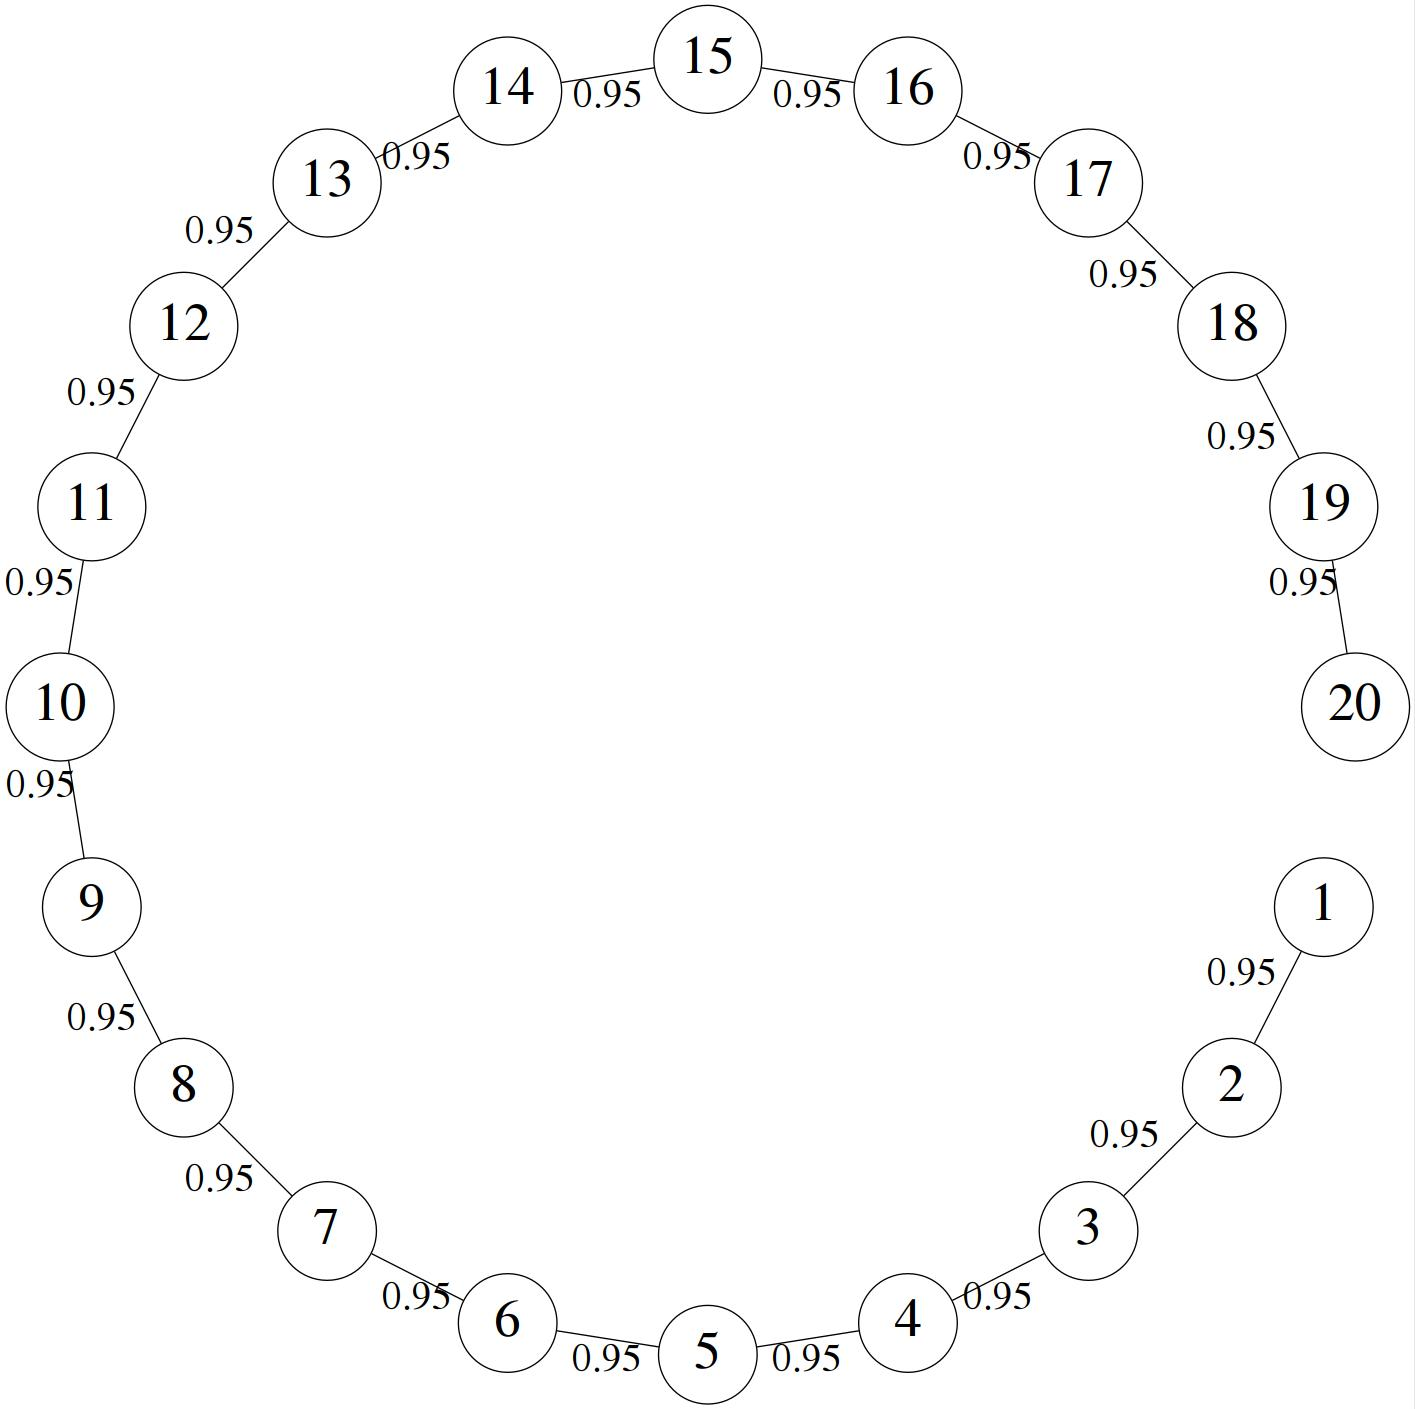
\includegraphics[width=0.8\linewidth]{graph.jpg}
\end{figure}

\newpage
\subsubsection{Test nr 2}
W teście nr 2 korzystamy z modelu podstawowego z dodatkowym połączeniem pomiędzy wierzchołkami 1 i 20 o niezawodności wynoszącej 0.95. Po wykonaniu symulacji uzyskujemy następujące wyniki:
\begin{table}[h!]
	\centering
    \label{tab:table1}
    \begin{tabular}{|c|c|c|c|}
    		\multicolumn{4}{c}{Liczba prób}\\
    		\hline
      	& 1,000,000 & 10,000,000 & 100,000,000\\
      	\hline
      	Niezawodność & 0.735969 & 0.735715 & 0.73583365\\
		\hline
    \end{tabular}
\end{table}

\noindent Model sieci:
\begin{figure}[h!]
	\centering
	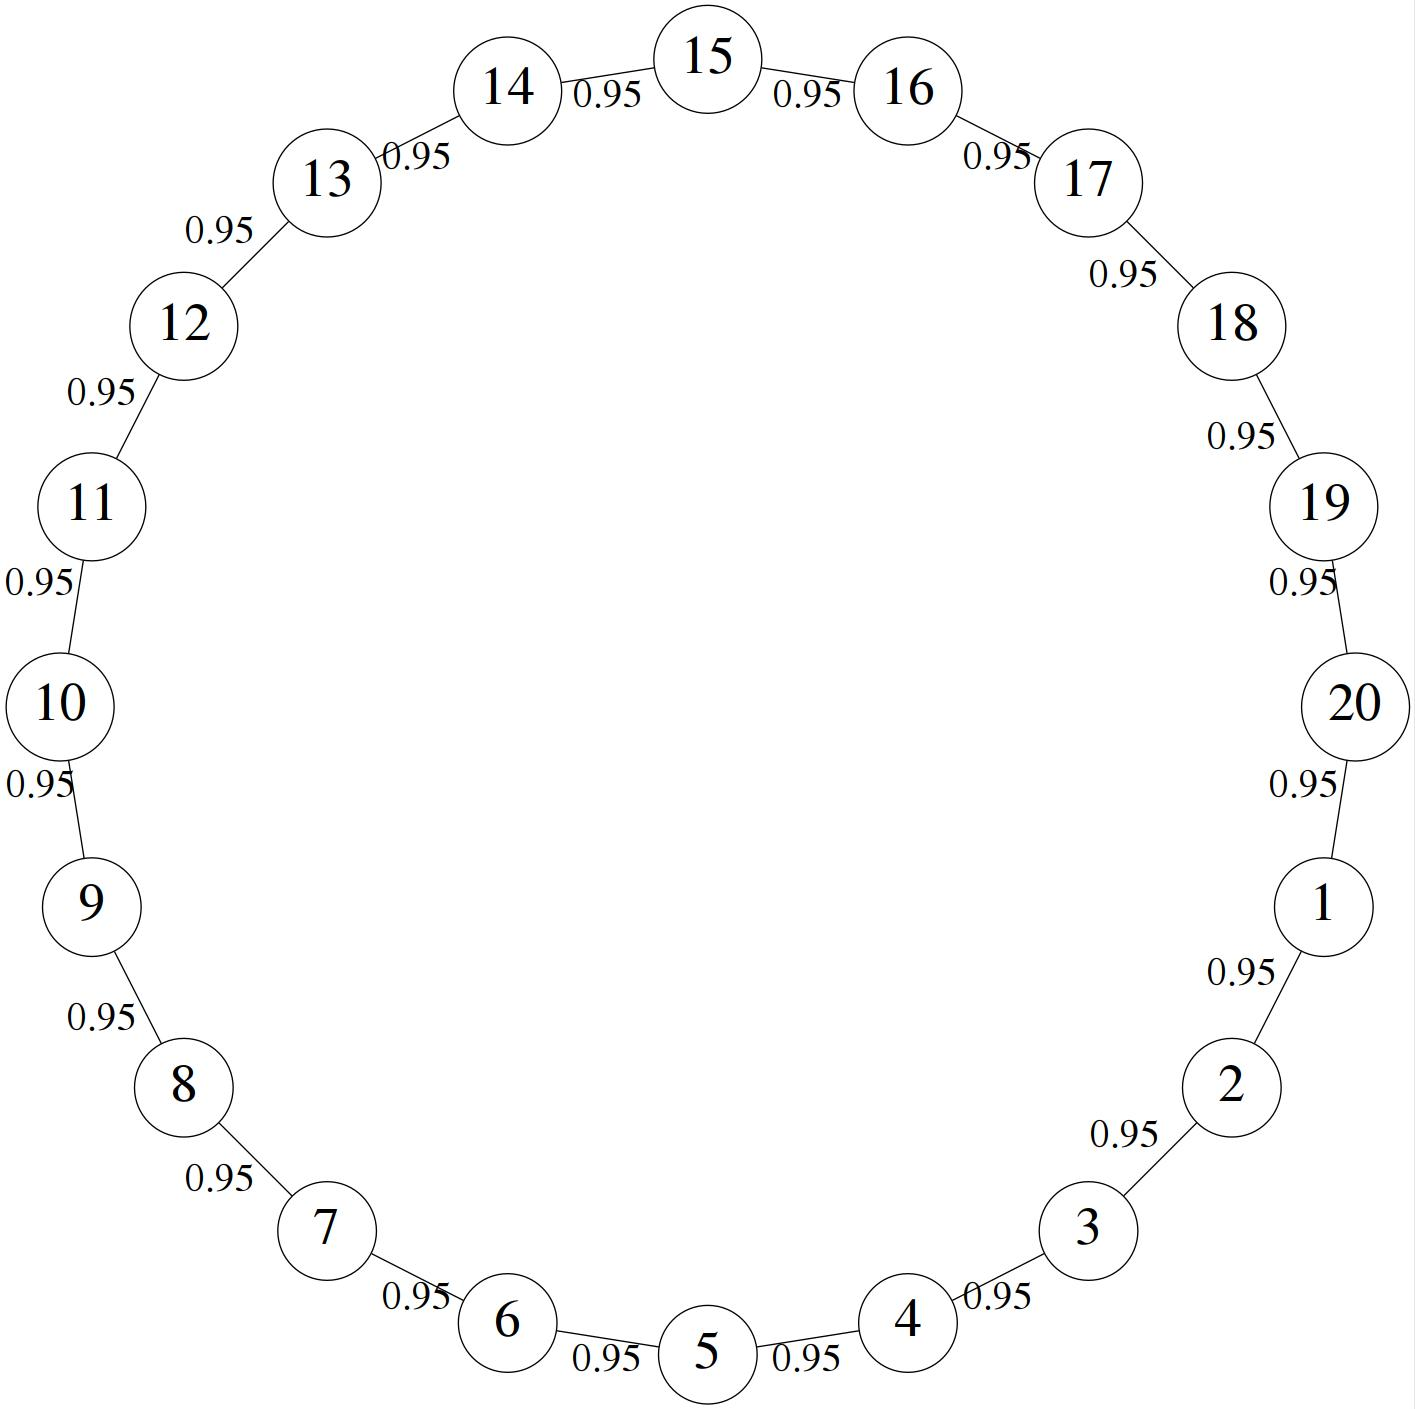
\includegraphics[width=0.8\linewidth]{graph2.jpg}
\end{figure}

\newpage
\subsubsection{Test nr 3}
W teście nr 3 korzystamy z modelu z poprzedniego test z dodatkowymi połączeniami pomiędzy wierzchołkami 1 i 10 oraz 5 i 15 o niezawodnościach wynoszących odpowiednio 0.8 i 0.7. Po wykonaniu symulacji uzyskujemy następujące wyniki:
\begin{table}[h!]
	\centering
    \label{tab:table1}
    \begin{tabular}{|c|c|c|c|}
    		\multicolumn{4}{c}{Liczba prób}\\
    		\hline
      	& 1,000,000 & 10,000,000 & 100,000,000\\
      	\hline
      	Niezawodność & 0.870627 & 0.8706126 & 0.87050279\\
		\hline
    \end{tabular}
\end{table}

\noindent Model sieci:
\begin{figure}[h!]
	\centering
	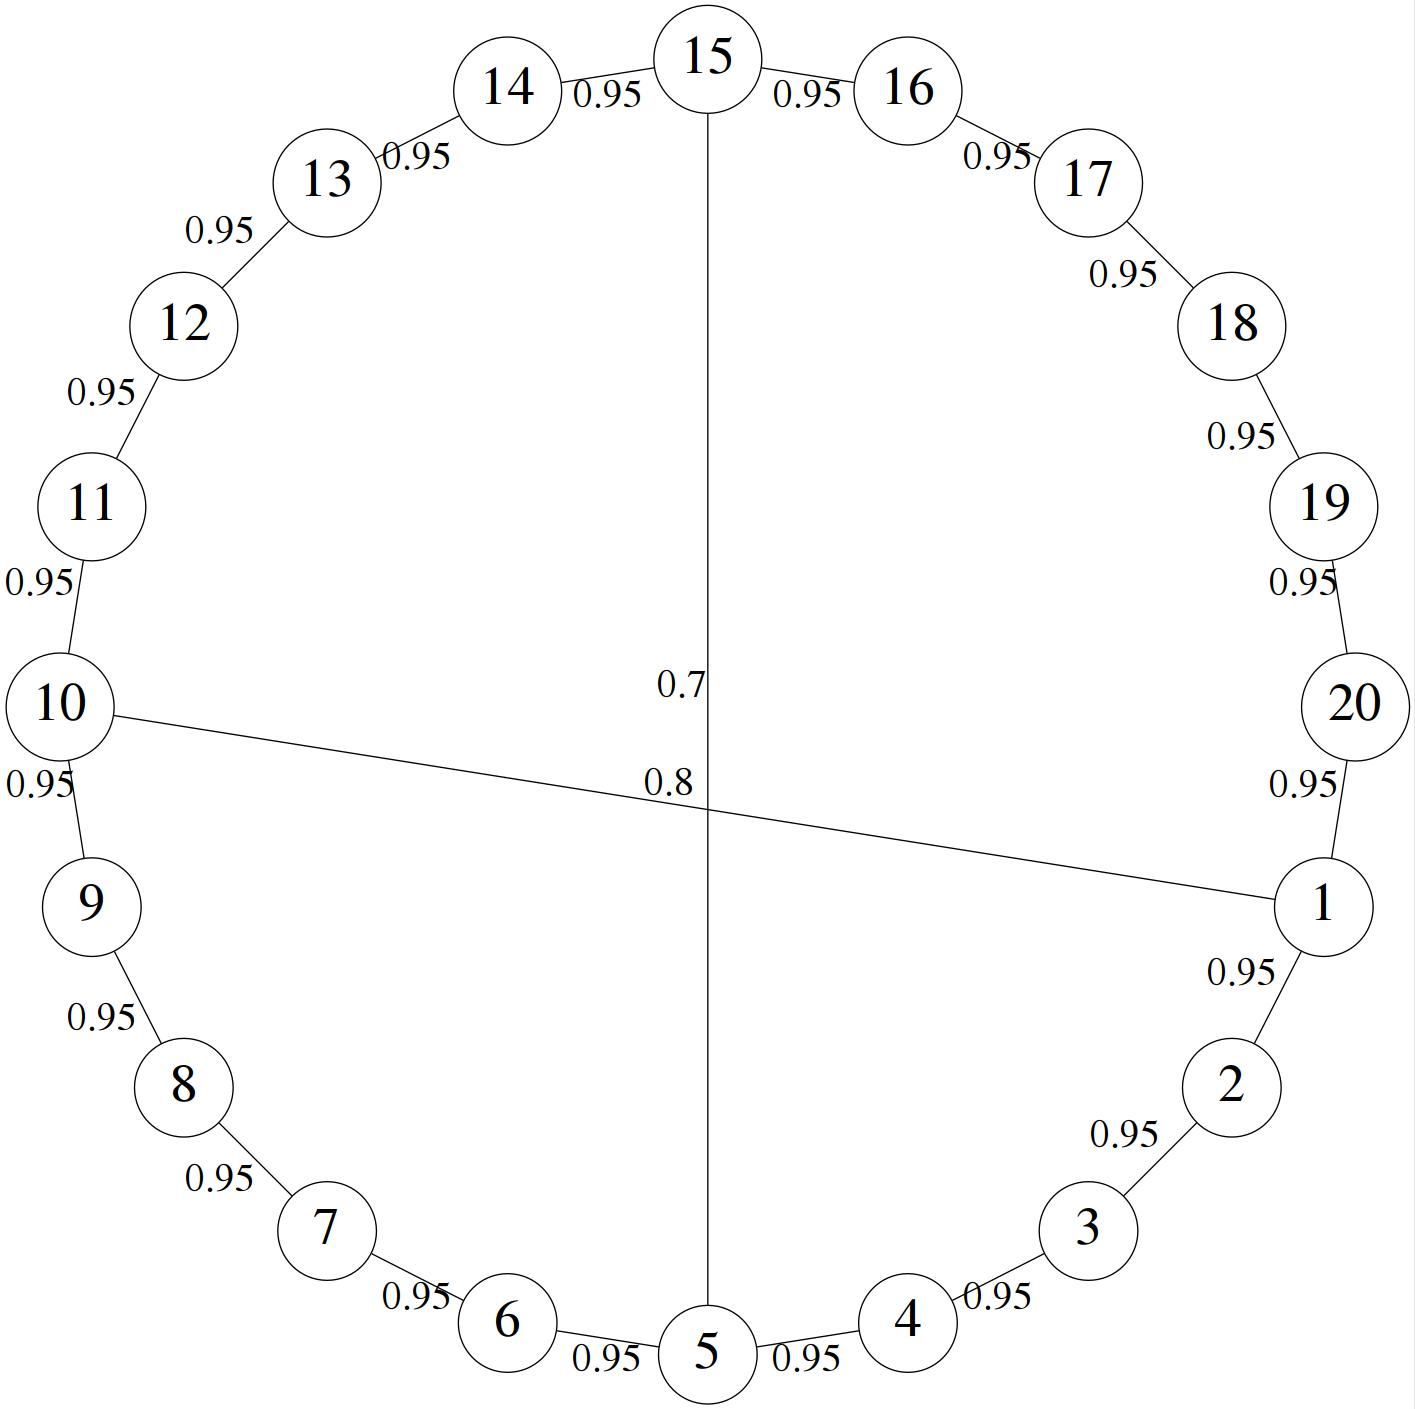
\includegraphics[width=0.8\linewidth]{graph3.jpg}
\end{figure}

\newpage
\subsubsection{Test nr 4}
W teście nr 4 korzystamy z modelu z poprzedniego testu z dodatkowymi dwoma połączeniami, o niezawodności wynoszącej $0.4$, pomiędzy losowymi wierzchołkami. Po wykonaniu symulacji uzyskujemy następujące wyniki:
\begin{table}[h!]
	\centering
    \label{tab:table1}
    \begin{tabular}{|c|c|c|c|}
    		\multicolumn{4}{c}{Liczba prób}\\
    		\hline
      	& 1,000,000 & 10,000,000 & 100,000,000\\
      	\hline
      	Niezawodność & 0.902696 & 0.9030207 & 0.90292538\\
		\hline
    \end{tabular}
\end{table}

\noindent Przykładowy model sieci:
\begin{figure}[h!]
	\centering
	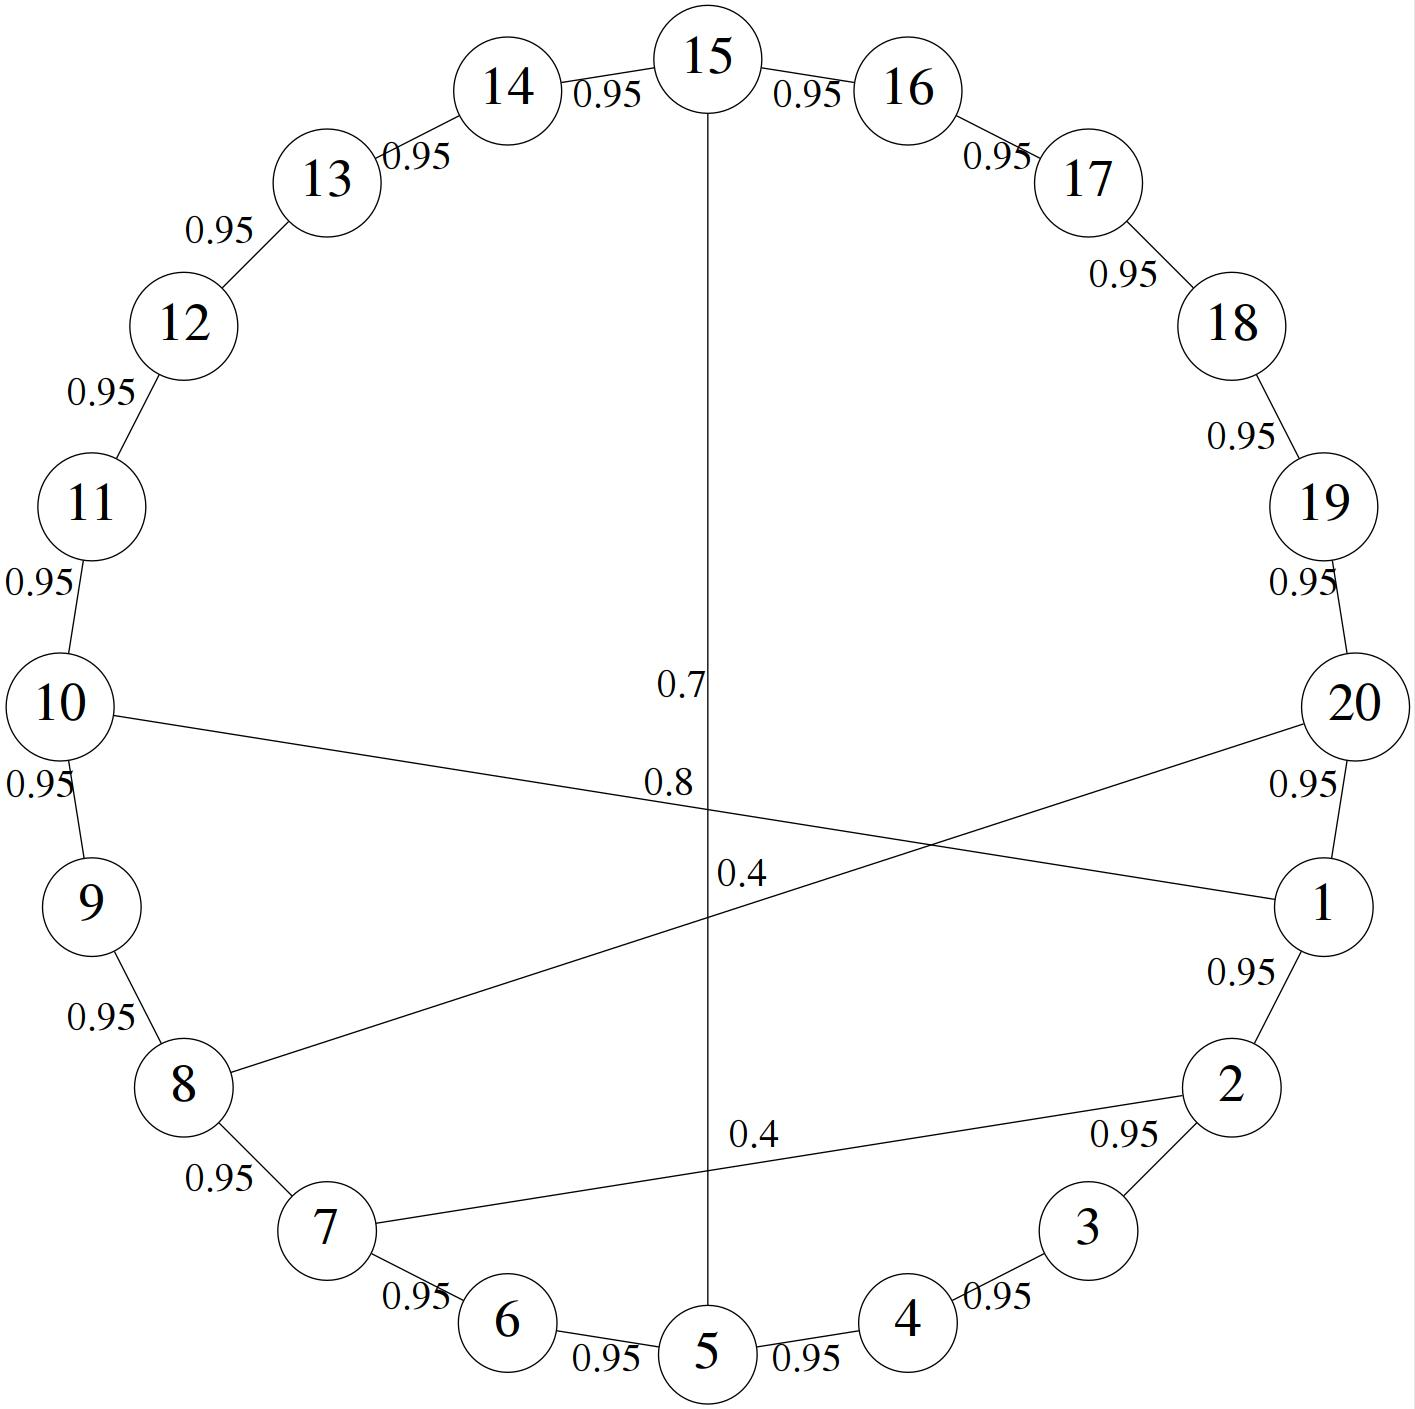
\includegraphics[width=0.8\linewidth]{graph4.jpg}
\end{figure}

\newpage
\subsection{Omówienie wyników}
Dla bardziej skomplikowanych sieci problemem jest analityczne policzenie niezawodności. Jednat dla sieci z testu nr 1 można obliczyć ją w prosty sposób. Sieć pozostaje spójna jeśli żaden z kanałów komunikacyjnych nie jest przerwany, czego prawdopodobieństwo wynosi $P = 0,95^{19} \approx 0.37735360$.

Obliczone prawdopodobieństwo jest bardzo zbliżone do uzyskanego wyniku, a na dokładność wpływa między innymi jakość użytego generatora pseudolosowego.

Jak można zauważyć, w teście nr 2, po dodaniu kanału pomiędzy wierzchołkami $1$ i $20$ prawdopodbieństwo znacząco wzrasta - wynika to z faktu, iż w modelu drugim po zniszczeniu jednego kanału komunikacyjnego sieć wciaż zachowuje spójność.

Podobnie w teście nr 3 i nr 4 dodawanie krawędzi zwiększa niezawodność sieci. W teście nr 4 na niezawodność sieci wpływa również to, które wierzchołki łączą wylosowane krawędzie - im większa odległość pomiędzy wolosowanymi wierzchołkami, tym większa niezawodność sieci.

\newpage
\section{Zadanie nr 2}

\end{document}